% Options for packages loaded elsewhere
\PassOptionsToPackage{unicode}{hyperref}
\PassOptionsToPackage{hyphens}{url}
\documentclass[
  catalan,
  a4paper,
]{article}
\usepackage{xcolor}
\usepackage[margin=1in]{geometry}
\usepackage{amsmath,amssymb}
\setcounter{secnumdepth}{-\maxdimen} % remove section numbering
\usepackage{iftex}
\ifPDFTeX
  \usepackage[T1]{fontenc}
  \usepackage[utf8]{inputenc}
  \usepackage{textcomp} % provide euro and other symbols
\else % if luatex or xetex
  \usepackage{unicode-math} % this also loads fontspec
  \defaultfontfeatures{Scale=MatchLowercase}
  \defaultfontfeatures[\rmfamily]{Ligatures=TeX,Scale=1}
\fi
\usepackage{lmodern}
\ifPDFTeX\else
  % xetex/luatex font selection
\fi
% Use upquote if available, for straight quotes in verbatim environments
\IfFileExists{upquote.sty}{\usepackage{upquote}}{}
\IfFileExists{microtype.sty}{% use microtype if available
  \usepackage[]{microtype}
  \UseMicrotypeSet[protrusion]{basicmath} % disable protrusion for tt fonts
}{}
\usepackage{setspace}
\makeatletter
\@ifundefined{KOMAClassName}{% if non-KOMA class
  \IfFileExists{parskip.sty}{%
    \usepackage{parskip}
  }{% else
    \setlength{\parindent}{0pt}
    \setlength{\parskip}{6pt plus 2pt minus 1pt}}
}{% if KOMA class
  \KOMAoptions{parskip=half}}
\makeatother
\usepackage{color}
\usepackage{fancyvrb}
\newcommand{\VerbBar}{|}
\newcommand{\VERB}{\Verb[commandchars=\\\{\}]}
\DefineVerbatimEnvironment{Highlighting}{Verbatim}{commandchars=\\\{\}}
% Add ',fontsize=\small' for more characters per line
\usepackage{framed}
\definecolor{shadecolor}{RGB}{248,248,248}
\newenvironment{Shaded}{\begin{snugshade}}{\end{snugshade}}
\newcommand{\AlertTok}[1]{\textcolor[rgb]{0.94,0.16,0.16}{#1}}
\newcommand{\AnnotationTok}[1]{\textcolor[rgb]{0.56,0.35,0.01}{\textbf{\textit{#1}}}}
\newcommand{\AttributeTok}[1]{\textcolor[rgb]{0.13,0.29,0.53}{#1}}
\newcommand{\BaseNTok}[1]{\textcolor[rgb]{0.00,0.00,0.81}{#1}}
\newcommand{\BuiltInTok}[1]{#1}
\newcommand{\CharTok}[1]{\textcolor[rgb]{0.31,0.60,0.02}{#1}}
\newcommand{\CommentTok}[1]{\textcolor[rgb]{0.56,0.35,0.01}{\textit{#1}}}
\newcommand{\CommentVarTok}[1]{\textcolor[rgb]{0.56,0.35,0.01}{\textbf{\textit{#1}}}}
\newcommand{\ConstantTok}[1]{\textcolor[rgb]{0.56,0.35,0.01}{#1}}
\newcommand{\ControlFlowTok}[1]{\textcolor[rgb]{0.13,0.29,0.53}{\textbf{#1}}}
\newcommand{\DataTypeTok}[1]{\textcolor[rgb]{0.13,0.29,0.53}{#1}}
\newcommand{\DecValTok}[1]{\textcolor[rgb]{0.00,0.00,0.81}{#1}}
\newcommand{\DocumentationTok}[1]{\textcolor[rgb]{0.56,0.35,0.01}{\textbf{\textit{#1}}}}
\newcommand{\ErrorTok}[1]{\textcolor[rgb]{0.64,0.00,0.00}{\textbf{#1}}}
\newcommand{\ExtensionTok}[1]{#1}
\newcommand{\FloatTok}[1]{\textcolor[rgb]{0.00,0.00,0.81}{#1}}
\newcommand{\FunctionTok}[1]{\textcolor[rgb]{0.13,0.29,0.53}{\textbf{#1}}}
\newcommand{\ImportTok}[1]{#1}
\newcommand{\InformationTok}[1]{\textcolor[rgb]{0.56,0.35,0.01}{\textbf{\textit{#1}}}}
\newcommand{\KeywordTok}[1]{\textcolor[rgb]{0.13,0.29,0.53}{\textbf{#1}}}
\newcommand{\NormalTok}[1]{#1}
\newcommand{\OperatorTok}[1]{\textcolor[rgb]{0.81,0.36,0.00}{\textbf{#1}}}
\newcommand{\OtherTok}[1]{\textcolor[rgb]{0.56,0.35,0.01}{#1}}
\newcommand{\PreprocessorTok}[1]{\textcolor[rgb]{0.56,0.35,0.01}{\textit{#1}}}
\newcommand{\RegionMarkerTok}[1]{#1}
\newcommand{\SpecialCharTok}[1]{\textcolor[rgb]{0.81,0.36,0.00}{\textbf{#1}}}
\newcommand{\SpecialStringTok}[1]{\textcolor[rgb]{0.31,0.60,0.02}{#1}}
\newcommand{\StringTok}[1]{\textcolor[rgb]{0.31,0.60,0.02}{#1}}
\newcommand{\VariableTok}[1]{\textcolor[rgb]{0.00,0.00,0.00}{#1}}
\newcommand{\VerbatimStringTok}[1]{\textcolor[rgb]{0.31,0.60,0.02}{#1}}
\newcommand{\WarningTok}[1]{\textcolor[rgb]{0.56,0.35,0.01}{\textbf{\textit{#1}}}}
\usepackage{longtable,booktabs,array}
\usepackage{calc} % for calculating minipage widths
% Correct order of tables after \paragraph or \subparagraph
\usepackage{etoolbox}
\makeatletter
\patchcmd\longtable{\par}{\if@noskipsec\mbox{}\fi\par}{}{}
\makeatother
% Allow footnotes in longtable head/foot
\IfFileExists{footnotehyper.sty}{\usepackage{footnotehyper}}{\usepackage{footnote}}
\makesavenoteenv{longtable}
\usepackage{graphicx}
\makeatletter
\newsavebox\pandoc@box
\newcommand*\pandocbounded[1]{% scales image to fit in text height/width
  \sbox\pandoc@box{#1}%
  \Gscale@div\@tempa{\textheight}{\dimexpr\ht\pandoc@box+\dp\pandoc@box\relax}%
  \Gscale@div\@tempb{\linewidth}{\wd\pandoc@box}%
  \ifdim\@tempb\p@<\@tempa\p@\let\@tempa\@tempb\fi% select the smaller of both
  \ifdim\@tempa\p@<\p@\scalebox{\@tempa}{\usebox\pandoc@box}%
  \else\usebox{\pandoc@box}%
  \fi%
}
% Set default figure placement to htbp
\def\fps@figure{htbp}
\makeatother
\ifLuaTeX
\usepackage[bidi=basic]{babel}
\else
\usepackage[bidi=default]{babel}
\fi
% get rid of language-specific shorthands (see #6817):
\let\LanguageShortHands\languageshorthands
\def\languageshorthands#1{}
\setlength{\emergencystretch}{3em} % prevent overfull lines
\providecommand{\tightlist}{%
  \setlength{\itemsep}{0pt}\setlength{\parskip}{0pt}}
\usepackage{bookmark}
\IfFileExists{xurl.sty}{\usepackage{xurl}}{} % add URL line breaks if available
\urlstyle{same}
\hypersetup{
  pdftitle={U6. EXEMPLE COMPTES, PERMISOS I PROPIETAT},
  pdfauthor={@tofermos 2026},
  pdflang={ca-ES},
  hidelinks,
  pdfcreator={LaTeX via pandoc}}

\title{U6. EXEMPLE COMPTES, PERMISOS I PROPIETAT}
\author{@tofermos 2026}
\date{}

\begin{document}
\maketitle

{
\setcounter{tocdepth}{2}
\tableofcontents
}
\setstretch{1.5}
\newpage
\renewcommand\tablename{Tabla}

\subsection{Problema}\label{problema}

En un taller de reparació, el tècnics han de guardar les fitxes de la
faena que fan en una carpeta on el gerent podrà consultar-les però no
modificar-les. \#\#\# Ordres

\begin{itemize}
\tightlist
\item
  useradd, groupadd, usermod, userdel
\item
  mkdir, touch
\item
  chown, chmod
\item
  ls, stat
\item
  id, cat, groups
\end{itemize}

\subsection{Solució.}\label{soluciuxf3.}

Com tenim un usuari -el gerent- amb uns permisos diferents (este serà el
U) i altres usuaris els agruparem en un grup (G). La resta d'usuaris (O,
others), per seguretat, no els deixarem ni accedir a la carpeta.
Recordeu que per llegir el contingut d'una carpeta, un usuari, ha de
tindre permís de lectura pero també d'execució per obrir-la.

\subsubsection{Pas 1. Crear els comptes}\label{pas-1.-crear-els-comptes}

Creem els comptes (usuaris i grups) que necessitem. * Usuari ``gerent''
* Grup ``tecnics'' (tecnci1, tecnic2\ldots)

\begin{Shaded}
\begin{Highlighting}[]
\ExtensionTok{tomas@portatil:\textasciitilde{}$}\NormalTok{ sudo useradd gerent }\AttributeTok{{-}md}\NormalTok{ /home/gerent}
\ExtensionTok{tomas@portatil:\textasciitilde{}$}\NormalTok{ sudo groupadd tecnics}
\ExtensionTok{tomas@portatil:\textasciitilde{}$}\NormalTok{ sudo useradd tecnic1 }\AttributeTok{{-}md}\NormalTok{ /home/tecnic1 }\AttributeTok{{-}g}\NormalTok{ tecnics}
\ExtensionTok{tomas@portatil:\textasciitilde{}$}\NormalTok{ sudo useradd tecnic2 }\AttributeTok{{-}md}\NormalTok{ /home/tecnic2 }\AttributeTok{{-}g}\NormalTok{ tecnics}
\ExtensionTok{tomas@portatil:\textasciitilde{}$}\NormalTok{ sudo passwd tecnic1}
\ExtensionTok{....}
\ExtensionTok{tomas@portatil:\textasciitilde{}$}\NormalTok{ sudo passwd tecnic2}
\end{Highlighting}
\end{Shaded}

\textbf{Si heu oblidat assignar el grup ( -g)} ``tecnics'' en la creació
de cada técnic podeu arreglar-ho \ldots{}

\ldots canviant-li el grup principal:

\begin{Shaded}
\begin{Highlighting}[]
\ExtensionTok{tomas@portatil:\textasciitilde{}$}\NormalTok{ sudo usermod tecnic1 }\AttributeTok{{-}g}\NormalTok{ tecnics}
\end{Highlighting}
\end{Shaded}

\ldots{} o afegir-los al grup sense llevar el que ja té de grup
principal (un usuari pot estar en molts grups)

\begin{Shaded}
\begin{Highlighting}[]
\ExtensionTok{tomas@portatil:\textasciitilde{}$}\NormalTok{ sudo usermod tecnic1 }\AttributeTok{{-}aG}\NormalTok{ tecnics}
\end{Highlighting}
\end{Shaded}

\textbf{Ara ja tenim els comptes creats!!}

\subsubsection{Pas 2. Creem la carpeta}\label{pas-2.-creem-la-carpeta}

⚠ Una carpeta compartida entre usuaris \textbf{MAI s'ha de crear dins
del perfil d'un usuari} /home/pep o (C:\users\pep, en Windows), per això
la creem en / o en /home

\begin{Shaded}
\begin{Highlighting}[]
\ExtensionTok{tomas@portatil:\textasciitilde{}$}\NormalTok{ mkdir /EMPRESA}
\ExtensionTok{mkdir:}\NormalTok{ no s’ha pogut crear el directori «/EMPRESA»: S’ha denegat el permís}
\end{Highlighting}
\end{Shaded}

NO ens permet crear perquè en el directori ``/'' sols pot escriure (w)
l'usuari root o qui puga emular-lo amb un sudo (o siga, els que
pertanyen al grup sudo) Comprovem-ho:

\begin{Shaded}
\begin{Highlighting}[]
\ExtensionTok{tomas@portatil:\textasciitilde{}$}\NormalTok{ ls }\AttributeTok{{-}ld}\NormalTok{ /}
\ExtensionTok{drwxr{-}xr{-}x}\NormalTok{ 24 root root 4096 de nov.  28 12:44 /}
\end{Highlighting}
\end{Shaded}

Per tant, caldrà executar el mkdir diguent-li al sistema que soc (usuari
tomas) un usuari sudoer (del grup sudo):

\begin{Shaded}
\begin{Highlighting}[]
\NormalTok{tomas@portatil:\textasciitilde{}$ sudo mkdir /EMPRESA}
\end{Highlighting}
\end{Shaded}

Compte! Hem creat la carpeta com sudoer, per tant tindrà assignat com a
propietari i grup principal \textbf{root:root}. Comprovem-ho:

\begin{Shaded}
\begin{Highlighting}[]
\NormalTok{tomas@portatil:\textasciitilde{}$ ls {-}ld /EMPRESA/}
\NormalTok{drwxr{-}xr{-}x 2 root root 4096 de nov.  28 12:44 /EMPRESA/}
\end{Highlighting}
\end{Shaded}

També podem comprovar-ho amb l'ordre \emph{stat}

\begin{Shaded}
\begin{Highlighting}[]
\NormalTok{tomas@portatil:\textasciitilde{}$ stat /EMPRESA/}
\NormalTok{  Fitxer: /EMPRESA/}
\NormalTok{       Mida: 4096       Blocs: 8          Bloc d’E/S: 4096   directori}
\NormalTok{Dispositiu: 10302h/66306d   Node‐i: 30932993    Enllaços: 2}
\NormalTok{Accés: (0755/drwxr{-}xr{-}x)  UID: (    0/    root)   GID: (    0/    root)}
\NormalTok{Accés: 2026{-}11{-}28 12:44:21.589258121 +0100}
\NormalTok{Modificació: 2026{-}11{-}28 12:44:21.589258121 +0100}
\NormalTok{      Canvi: 2026{-}11{-}28 12:44:21.589258121 +0100}
\NormalTok{  Naixement: 2026{-}11{-}28 12:44:21.589258121 +0100}
\end{Highlighting}
\end{Shaded}

\subsubsection{Pas 3. Canviem el propietari i grup principal de la
carpeta
(chown)}\label{pas-3.-canviem-el-propietari-i-grup-principal-de-la-carpeta-chown}

Abans d'assignar permisos, hem de saber \textbf{a qui} anem a
assignar-los. Ja hem vist que la carpeta és de l'usuari 0 (root) i té el
grup 0 (root) com grup principal: els hem de canviar als que necessitem.

\begin{Shaded}
\begin{Highlighting}[]
\ExtensionTok{tomas@portatil:\textasciitilde{}$}\NormalTok{ sudo chown gerent:tecnics /EMPRESA}
\end{Highlighting}
\end{Shaded}

Comprovem el canvi amb el `ls -ld' i també amb `stat'

\begin{Shaded}
\begin{Highlighting}[]
\ExtensionTok{tomas@portatil:\textasciitilde{}$}\NormalTok{ ls }\AttributeTok{{-}ld}\NormalTok{ /EMPRESA/}
\ExtensionTok{drwxr{-}xr{-}x}\NormalTok{ 2 gerent tecnics 4096 de nov.  28 12:44 /EMPRESA/}
\ExtensionTok{tomas@portatil:\textasciitilde{}$}\NormalTok{ stat /EMPRESA/}
\ExtensionTok{Fitxer:}\NormalTok{ /EMPRESA/}
       \ExtensionTok{Mida:}\NormalTok{ 4096       Blocs: 8          Bloc d’E/S: 4096   directori}
\ExtensionTok{Dispositiu:}\NormalTok{ 10302h/66306d   Node‐i: 30932993    Enllaços: 2}
\ExtensionTok{Accés:} \ErrorTok{(}\ExtensionTok{0755/drwxr{-}xr{-}x}\KeywordTok{)}  \ExtensionTok{UID:} \ErrorTok{(} \ExtensionTok{1004/}\NormalTok{  gerent}\KeywordTok{)}   \ExtensionTok{GID:} \ErrorTok{(} \ExtensionTok{1013/}\NormalTok{ tecnics}\KeywordTok{)}
\ExtensionTok{Accés:}\NormalTok{ 2026{-}11{-}28 12:44:21.589258121 +0100}
\ExtensionTok{Modificació:}\NormalTok{ 2026{-}11{-}28 12:44:21.589258121 +0100}
      \ExtensionTok{Canvi:}\NormalTok{ 2026{-}11{-}28 13:15:34.715863906 +0100}
  \ExtensionTok{Naixement:}\NormalTok{ 2026{-}11{-}28 12:44:21.589258121 +0100}
\end{Highlighting}
\end{Shaded}

\subsubsection{Pas 4. Assignem permisos
(chmod)}\label{pas-4.-assignem-permisos-chmod}

Ara que la carpeta té el usuari i el grup adient, ja podem donar-los els
permisos:

\begin{itemize}
\tightlist
\item
  Un grup d'usuaris ``tecnics'' que tindrà permís de \textbf{lectura
  (r), escriptura (w) i execució (x)}
\item
  L'usuari ``gerent'' només podrà llegir en la carpeta:
  \textbf{lectura(r) i execució (x)}
\end{itemize}

\begin{Shaded}
\begin{Highlighting}[]
\NormalTok{tomas@portatil:\textasciitilde{}$ sudo chmod 570 /EMPRESA}
\end{Highlighting}
\end{Shaded}

Ho comprovem

\begin{Shaded}
\begin{Highlighting}[]
\ExtensionTok{tomas@portatil:\textasciitilde{}$}\NormalTok{ ls }\AttributeTok{{-}ld}\NormalTok{ /EMPRESA/}
\ExtensionTok{dr{-}xrwx{-}{-}{-}}\NormalTok{ 2 gerent tecnics 4096 de nov.  28 12:44 /EMPRESA/}
\ExtensionTok{tomas@portatil:\textasciitilde{}$}\NormalTok{ stat /EMPRESA/}
  \ExtensionTok{Fitxer:}\NormalTok{ /EMPRESA/}
       \ExtensionTok{Mida:}\NormalTok{ 4096       Blocs: 8          Bloc d’E/S: 4096   directori}
\ExtensionTok{Dispositiu:}\NormalTok{ 10302h/66306d   Node‐i: 30932993    Enllaços: 2}
\ExtensionTok{Accés:} \ErrorTok{(}\ExtensionTok{0570/dr{-}xrwx{-}{-}{-}}\KeywordTok{)}  \ExtensionTok{UID:} \ErrorTok{(} \ExtensionTok{1004/}\NormalTok{  gerent}\KeywordTok{)}   \ExtensionTok{GID:} \ErrorTok{(} \ExtensionTok{1013/}\NormalTok{ tecnics}\KeywordTok{)}
\ExtensionTok{Accés:}\NormalTok{ 2026{-}11{-}28 12:44:21.589258121 +0100}
\ExtensionTok{Modificació:}\NormalTok{ 2026{-}11{-}28 12:44:21.589258121 +0100}
      \ExtensionTok{Canvi:}\NormalTok{ 2026{-}11{-}28 13:21:48.836791095 +0100}
  \ExtensionTok{Naixement:}\NormalTok{ 2026{-}11{-}28 12:44:21.589258121 +0100}
\end{Highlighting}
\end{Shaded}

\begin{longtable}[]{@{}
  >{\raggedright\arraybackslash}p{(\linewidth - 8\tabcolsep) * \real{0.0741}}
  >{\centering\arraybackslash}p{(\linewidth - 8\tabcolsep) * \real{0.1481}}
  >{\centering\arraybackslash}p{(\linewidth - 8\tabcolsep) * \real{0.1481}}
  >{\raggedright\arraybackslash}p{(\linewidth - 8\tabcolsep) * \real{0.1111}}
  >{\raggedright\arraybackslash}p{(\linewidth - 8\tabcolsep) * \real{0.5185}}@{}}
\toprule\noalign{}
\begin{minipage}[b]{\linewidth}\raggedright
De qui?
\end{minipage} & \begin{minipage}[b]{\linewidth}\centering
Octal
\end{minipage} & \begin{minipage}[b]{\linewidth}\centering
Binari(intern)
\end{minipage} & \begin{minipage}[b]{\linewidth}\raggedright
Descripció
\end{minipage} & \begin{minipage}[b]{\linewidth}\raggedright
\end{minipage} \\
\midrule\noalign{}
\endhead
\bottomrule\noalign{}
\endlastfoot
U & 5 & 101 & r-x & Pot entrar a la carpeta i llegir (vore) els
fitxers \\
G & 7 & 111 & rwx & Poden entrar a la carpeta vore, crear, modificar o
eliminar fitxers \\
O & 0 & 000 & --- & No poden obrir ni entrar a la carpeta \\
\end{longtable}

\subsubsection{Pas 5. Comprovació.}\label{pas-5.-comprovaciuxf3.}

Per fer la prova podem iniciar sessions dels diferents usuaris amb
\textbf{su/exit}

\begin{figure}
\centering
\pandocbounded{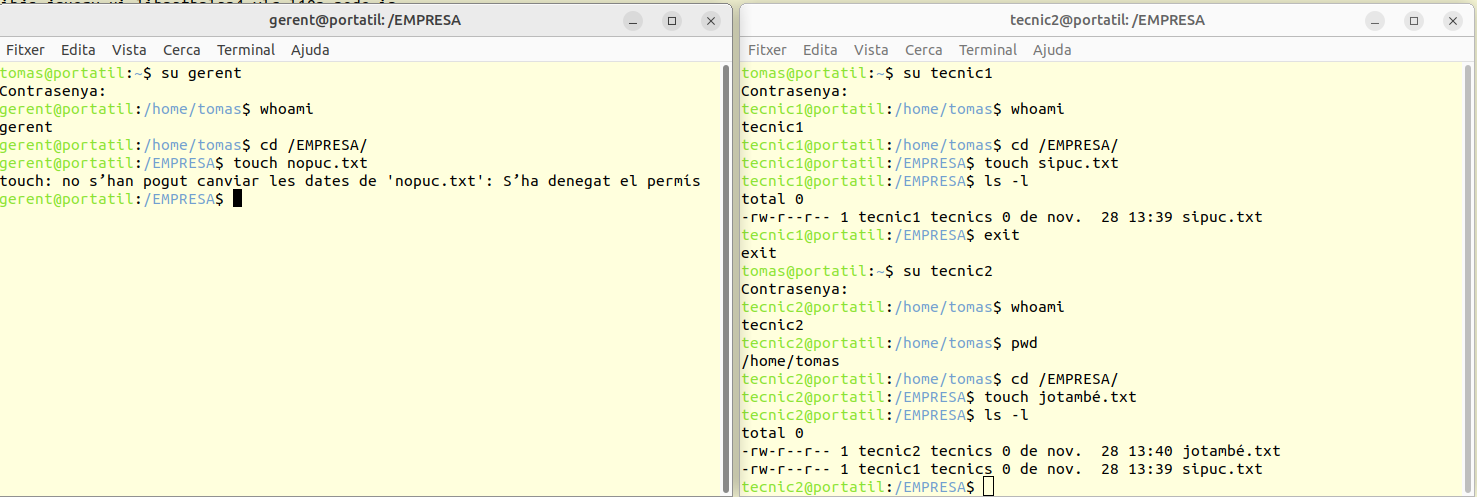
\includegraphics[keepaspectratio]{png/gerenttecnics.png}}
\caption{Comprovació}
\end{figure}

\end{document}
